%\documentclass[a4paper,11pt,twoside]{article}
\documentclass[preprint,10pt,numbers]{sigplanconf}
\usepackage[utf8]{inputenc}          % UTF-8 Encoding
\usepackage{hyperref}                % Interactive PDF
\usepackage{float}                   % Float control
\usepackage{caption}                 
\usepackage{subcaption}
\usepackage{multirow}                % Span multiple rows & columns in a table
\usepackage{amsmath}                 % Mathematics library
\usepackage{amssymb}                 % Provides math fonts
\usepackage{amsthm}                  % Provides \newtheorem, \theoremstyle, etc.
\usepackage[T1]{fontenc}             % Fixes font issues
\usepackage{lmodern}
\usepackage{tikz}                    % Drawing
\usetikzlibrary{trees}
\usetikzlibrary{calc}
\usepackage{xcolor}
\usepackage{listings}

\lstset{
 backgroundcolor=\color{white},   % choose the background color; you must add \usepackage{color} or \usepackage{xcolor}
 basicstyle=\ttfamily\small,        % the size of the fonts that are used for the code
 commentstyle=\itshape,
 breakatwhitespace=false,         % sets if automatic breaks should only happen at whitespace
 breaklines=true,                 % sets automatic line breaking
 captionpos=b,                    % sets the caption-position to bottom
 deletekeywords={...},            % if you want to delete keywords from the given language
 escapeinside={(*}{*)},          % if you want to add LaTeX within your code
 extendedchars=true,              % lets you use non-ASCII characters; for 8-bits encodings only, does not work with UTF-8
 frame=none,	                   % adds a frame around the code
 keepspaces=true,                 % keeps spaces in text, useful for keeping indentation of code (possibly needs columns=flexible)
 numbers=none,                    % where to put the line-numbers; possible values are (none, left, right)
 rulecolor=\color{black},         % if not set, the frame-color may be changed on line-breaks within not-black text (e.g. comments (green here))
 showspaces=false,                % show spaces everywhere adding particular underscores; it overrides 'showstringspaces'
 showstringspaces=false,          % underline spaces within strings only
 showtabs=false,                  % show tabs within strings adding particular underscores
 tabsize=2,	                   % sets default tabsize to 2 spaces
 title=\lstname,                   % show the filename of files included with \lstinputlisting; also try caption instead of title
  belowcaptionskip=-1\baselineskip,
  xleftmargin=\parindent
}
% Links style
\lstdefinestyle{links}{
  basicstyle=\linespread{1.0}\ttfamily\footnotesize,
  language=Caml,
  frame=none,
  literate= {+}{{$+$}}1 {*}{{$*$}}1
            {<=}{{$\leq$}}1 {>=}{{$\geq$}}1 
            {=>}{{$\Rightarrow$}}1
            {->}{{$\to$}}1 {~>}{{$\rightsquigarrow$}}1
}
%\usepackage[
%backend=bibtex,
%style=numeric,
%sorting=nyt
%]{biblatex}                   % Bibliography
%\addbibresource{references.bib}


% Convenient macros
\newcommand{\defas}[0]{\mathrel{\overset{\makebox[0pt]{\mbox{\normalfont\tiny\sffamily def}}}{=}}} % "defined-as-equal"

%% Meta-stuff like authors, title, etc.
%\author{Daniel Hillerström\\\small{CDT in Pervasive Parallelism}\\\small{\href{mailto:daniel.hillerstrom@ed.ac.uk}{daniel.hillerstrom@ed.ac.uk}}}
%\date{\today}
%\title{Proposal: Effective Concurrency in Links} % Just some title; change at a later point.

% The document
\makeatletter
\def\@copyrightspace{\relax}
\makeatother
\begin{document}
\title{Proposal: Modular and Effective Concurrency in Links}
%\subtitle{via handlers}

\authorinfo{Daniel Hillerström}
           {CDT Pervasive Parallelism}
           {\href{mailto:daniel.hillerstrom@ed.ac.uk}{daniel.hillerstrom@ed.ac.uk}}
  \maketitle
  \begin{abstract}
Efficient task scheduling is important in order to achieve performance. Yet the programmer's influence on scheduling is limited, because existing programming models often provide weak abstractions which lack modularity. 
%The choice of scheduling strategy affects the performance of application. But often the programmer has little or no influence on the matter. There exists many tools that address this mismatch for high-performance computing. However, these tools require the programmer to describe programs in a foreign language which renders code non-modular.

We propose a novel, efficient implementation of effect handlers in Links that uses a resource-tracking type system to enable a code generator specialise the run-time implementation of individual handlers. Furthermore, we hypothesise that we can achieve ``concurrency for free'' by encoding concurrency primitives via handlers.
  \end{abstract}
  %\raggedbottom
  % Input the content
  \section{Introduction}
Run-time scheduling is a domain-specific problem as the performance goal of a scheduler can be paramount to the overall performance of a program. For example, system schedulers seek to optimise the job throughput. Resource schedulers attempt to ensure fairness by coordinating accesses to shared resources. Task schedulers seek to reduce execution time by considering factors such as dependencies among tasks. In addition, task schedulers may also seek to exploit special-purpose accelerators in the environment in order to speed up task execution.

% Many different domains, we want modularity

%Consequently, schedulers employ different metrics to measure performance. For example, \emph{high-throughput} schedulers seek to optimise the throughput of jobs \cite{Berman2003}, hence performance might be measured by the number of jobs processed by the system. Criteria such as fairness or utilisation might be used to measure the performance of \emph{resource} schedulers as they seek to coordinate accesses to shared resources \cite{Berman2003}. Furthermore, \emph{high-performance} schedulers seek to minimise execution time for a single program. In this case performance is measured by the raw execution speed.

In most programming models the programmer has little or no say regarding scheduling. Unfortunately, the schedulers are often tightly coupled with a generic run-time system. Thus, scheduling is responsibility of the run-time implementor, but the concern of the application programmer \cite{Dolan2015}. 
%For example, the application programmer's knowledge of the problem domain may accelerate program execution grid-based computations may benefit from neighbouring points being scheduled together. Yet the programmer has little or no say about the matter as schedulers typically are baked into the run-time system \cite{Dolan2015}. 

We propose to rectify this mismatch by transferring the responsibility for scheduling to the application programmer. Concretely, we propose to abstract over the choice of scheduling by adapting the approach taken by Multicore OCaml \cite{Dolan2015} to use Plotkin and Pretnar's \emph{handlers for algebraic effects} \cite{Plotkin2013} to encode scheduling primitives. Specifically, we plan implement a backend for the functional programming language Links \cite{Cooper2006}, and take advantage of its existing implementation of algebraic effect handlers \cite{Hillerstrom2015} to encode Links' concurrency primitives.

  % Plotkin and Power's algebraic effects \cite{Plotkin2001} combined with Plotkin and Pretnar's handlers \cite{Plotkin2013} yield a programming model for controlling computational effects. An algebraic effect is a collection of abstract operations without predefined semantics. Handlers interpret algebraic effects by assigning semantics to abstract operations. Thus, the control of computational effects is lifted from the run-time system into the hands of the programmer. Clearly, it shifts additional responsibility onto the programmer, however, in addition it opens up a design space that was previously secluded from the programmer. Now, the programmer may extend the capabilities of the run-time system beyond what the language implementor envisaged.

  % For example, it is well-known that concurrency primitives can be encoded through algebraic effects \cite{Bauer2015,Dolan2015} as spawning a new thread is an effect. Furthermore, suspending a thread is an effect. Handlers of these effects are schedulers. Hence, the programmer is free to implement a particular scheduling policy tailored for the application. The choice of scheduler can have significant impact on performance as a scheduler's performance goal can be paramount to the overall performance of an application \cite{Berman2003}.

  % However\dots

  \section{Problem definition}\label{sec:problemdefinition}
%  Although, handlers for algebraic effects have many practical applications \cite{Kammar2013,Bauer2015,Hillerstrom2015,Dolan2015}, there does not yet exist an efficient implementation of handlers. Multicore OCaml implements linear handlers which only allow the continuation invoked once. This restriction is enforced during run-time. Furthermore, because OCaml lacks an effect system\dots
%Run-time scheduling is recognised as an important problem for performance \cite{Augonnet2011,Augonnet2012,Agullo2015,Openmp2013}. 
There exists many concurrent and parallel programming models that attempt to involve programmer participation in scheduling, e.g. CellSs \cite{Bellens2009}, StarSs \cite{Planas2009}, StarPU \cite{Augonnet2011}, OpenMP \cite{Openmp2013} and PaRSEC \cite{Bosilca2013} to mention a few.\footnote{These tools are further discussed in Section \ref{sec:relatedwork}.}

These models operate on task graph based descriptions of programs. They will try to map individual tasks onto computational devices automatically.

However, the key observation is, that, the aforementioned tools provide weak abstractions that makes scheduling non-modular. Support for schedulers is added by resorting to compile-time meta programming in a foreign language such as \texttt{\#pragmas}. As a consequence scheduling strategies and tasks become tightly coupled. In addition, it becomes nontrivial to swap scheduling strategies.
% Moreover, the programmer still has a limited say.
% End up with a monolithic tools

Ideally, we would want schedulers to be first-class citizens in the host language. Therefore, we ask the following question:
\begin{center}
  \emph{How may we reify schedulers as an integrated host language construct?}
\end{center}
In Section \ref{sec:proposedsolution} we propose an answer to the above question.

\section{Background}\label{sec:background}
In Section \ref{sec:effects-and-handlers} introduces algebraic effects and handlers, while Section \ref{sec:effect-links} introduces an implementation of them in the functional programming language Links.

\subsection{Algebraic effects and their handlers}\label{sec:effects-and-handlers}
Plotkin and Power introduced algebraic effects \cite{Plotkin2001} for modelling the semantics of effectful computations \cite{Lindley2014}. An algebraic effect is a collection of abstract operations. For example, we might define an algebraic effect for state: $State(s) \defas \{Get:s,Put:s \to ()\}$. State is an effect with two operations: Get and Put which retrieves and modify some state $s$, respectively. The State effect and its operations do not have predefined semantics.

\begin{figure*}[t!]
\begin{subfigure}[b]{0.5\textwidth}
\centering
\begin{lstlisting}[caption={},style=links]
sig withdraw : (*$(\texttt{Int}) \xrightarrow{\texttt{\{Get:Int},\texttt{Put:(Int)} \to ()|\varepsilon\}} \texttt{Int}$*)
fun withdraw(amount) {
  var balance = get();
  if (balance - amount > 0) {
    put(balance - amount); amount
  } else {
    0
  }
}
\end{lstlisting}
\caption{Computation tree for \dots}\label{fig:effecttree}
\end{subfigure}
~
\begin{subfigure}[b]{0.5\textwidth}
\centering
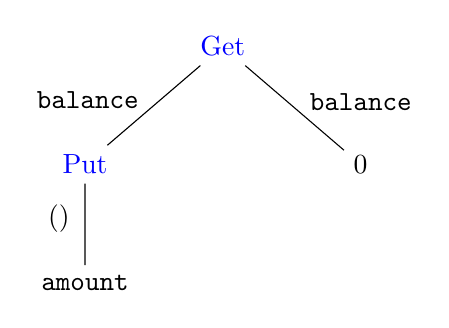
\begin{tikzpicture}[level distance=1.5cm,
level 1/.style={sibling distance=3.5cm},
level 2/.style={sibling distance=2cm}]
%\tikzstyle{every node}=[circle,draw]

\node (Root) [blue,rectangle] {Get}
    child { node[blue] (q0) {Put} 
      child { node[draw=none] (q00) {\texttt{amount}}
        edge from parent node [draw=none,left,xshift=-2.0,yshift=2.0] {()}
      }      
      edge from parent node [draw=none,left,xshift=-2.0,yshift=2.0] {\texttt{balance}}
    }
    child { node [draw=none] (q1) {0}
      edge from parent node [draw=none,right,xshift=2.0,yshift=2.0] {\texttt{balance}}
    };
\end{tikzpicture}
\caption{Computation tree for \dots}\label{fig:effecttree}
\end{subfigure}
\caption{Computation and its computation tree.}
\end{figure*}

Handlers assign semantics to effects. Essentially, handlers interpret invocations of abstract operations in computations. Handlers may be either closed or open. A closed handler handles a fixed set of effects, whilst an open handler handles a subset of effects. Open handlers can be composed together to handle a larger set of effects. In addition, handlers comes in two different flavours: \emph{deep} or \emph{shallow}.

% Intuitively handlers fold computation trees

%\subsection{Continuations}\label{sec:continuations}

  \subsection{Links with effect handlers}\label{sec:effect-links}
  Links is a strongly, statically and structural typed functional programming language \cite{Cooper2006}. Notably, Links implements effect handlers as first-class citizens \cite{Hillerstrom2015}. Intuitively, handlers are interpreters that pattern matches on abstract operations occurring in handled computation. This is directly reflected in the syntax for handlers; for example the following handler handles stateful computations that modify program state \texttt{s} via two operations $\texttt{get} : s$ and $\texttt{put} : s \to ()$:
\begin{lstlisting}[style=links,caption={}]
sig state : (*$\left(() \xrightarrow{\{Get:s,Put:s\to()\}} a\right) \to (s) \to a$*)
handler state(m)(s) {
  case Get(k)    -> k(s)(s)
  case Put(p,k)  -> k(())(p)
  case Return(x) -> x
}
\end{lstlisting}
The signature for \texttt{state} conveys that it handles some computation \texttt{m} whose effect signature contains (only) \texttt{Get} and \texttt{Put}, the computation returns a value of type \texttt{a}. The second parameter \texttt{s} is the program state which the computation \texttt{m} may modify.
The case-statements pattern matches on the operation names in effect signature of \texttt{m}.
The cases \texttt{Get} and \texttt{Put} matches on user-defined operations, while the \texttt{Return} operation is a special, built-in operation that is invoked implicitly, when the computation \texttt{m} returns.

When an operation is invoked in \texttt{m} the run-time generates a continuation from that point in the program. Then the run-time transfers control to the handler which exposes this continuation is to the programmer via the parameter \texttt{k} in the case-statements. For example, when \texttt{Get} is invoked this particular handler invokes the continuation with the current state \texttt{s}. This effectively resumes the computation \texttt{m} with the state \texttt{s}. Moreover, the same state \texttt{s} is forwarded to the next invocation of the handler. In the case of \texttt{Put}, the handler invokes the continuation with unit, and forwards the new state \texttt{p}.


At the time of writing effect handlers are only supported by the Links interpreter. Thus the performance of handlers is low.

  \section{Proposed solution}\label{sec:proposedsolution}
%The main observation is, that, tools often happen to offer poor abstractions which requires the programmer to annotate or describe code in \emph{a foreign language}. As a consequence code becomes non-modular, and thus, it difficult to combine different pieces of code.
We advocate an approach along the lines of Multicore OCaml to use algebraic effect handlers to encode concurrency directly in the host language. Plotkin and Power's algebraic effects \cite{Plotkin2001} are collections of abstract operations without predefined semantics. Plotkin and Pretnar's handlers \cite{Plotkin2013} assign semantics to abstract operations. Thus this programming model provide a clear separation of computational effects and their interpretations.

The key observation is that concurrent and parallel concepts such as task forking, kernel launch and data-sharing are effects \cite{Bauer2015,Dolan2015}. Hence, concurrency is encodable through algebraic effects \cite{Bauer2015,Dolan2015}. Handlers (interpretations) for these effects implement scheduling strategies. Sections \ref{sec:eff} and \ref{sec:sched} give a concrete example of a possible encoding of asynchronous task, and two possible task schedulers.

\subsection{Encoding cooperative multitasking}\label{sec:eff}
We may encode \emph{cooperative multitasking} using the following two operations:
\begin{itemize}
  \item $\text{fork} : (() \to a) \to F a$
  \item $\text{yield} : ()$
\end{itemize}
The first operation \emph{fork} takes a task as input, and returns a future which eventually will contain the result of the said task. The second operation \emph{yield} suspends the task which it is invoked inside. Using these operations we can easily define an asynchronous computation that computes the $n$th Fibonacci number, e.g. 
\begin{lstlisting}[style={links},caption={}]
fun fib(n) {
  if (n <= 1) {n}
  else {
    var f1 = fork(fun() { fib(n-1) });
    var f2 = fork(fun() { fib(n-2) });
    get(f1) + get(f2)
  }
}
\end{lstlisting}
where \texttt{get} attempts to retrieve the value inside a future. Its implementation is omitted here, but it is simple to implement in terms of yield.\footnote{The full source code is available at \url{https://github.com/dhil/mscr-dissertation/proposal/coroutines.links}} 

\subsection{Scheduling tasks}\label{sec:sched}
Next, we define a scheduler:
\begin{lstlisting}[style={links},caption={}]
open handler sched(m)(f) {
  case Fork(t,k) -> {
   var new_f = new_future();
   enqueue(fun(_){sched(t)(Just(new_f))()});
   k(new_f)(f)
  }
  case Yield(k)  -> { 
   enqueue(fun(_) { k(())(f) }); 
   var t = dequeue(); t(()) 
  }
  case Return(x) -> {
     put(f,x);
     if (is_empty()) { x }
     else { var t = dequeue(); t(()) }
   } 
}
\end{lstlisting}
The handler \texttt{bfscheduler} implements a scheduler by pattern matching on occurrences of operations \texttt{Fork} and \texttt{Yield} in some computation \texttt{m}. The handler is parameterised by a future \texttt{f}. For instance, when \texttt{fork} occurs in \texttt{fib} the \texttt{bfscheduler} first allocates a new future \texttt{new\_f}. Then it recursively schedules the forked task \texttt{t} to run later. Finally, it resumes the task in which \texttt{t} was forked by invoking the continuation \texttt{k} with the new future \texttt{new\_f}, the previous future \texttt{f} is saved for the next invocation of the scheduler. Observe, that on a single-core platform this scheduler effectively defers execution of forked tasks.

Upon an occurrence of \texttt{yield} in \texttt{m} the handler suspends the task and schedules it to run later. Thereafter it dequeues and resumes another task \texttt{t}.

Finally, when a task finishes the handler puts the return value inside the future \texttt{f}. Furthermore, if the task queue is nonempty it dequeues and resumes another task, otherwise it the return value of latest task is returned.
\begin{figure*}[t!]
\begin{subfigure}[t]{0.5\textwidth}
\centering
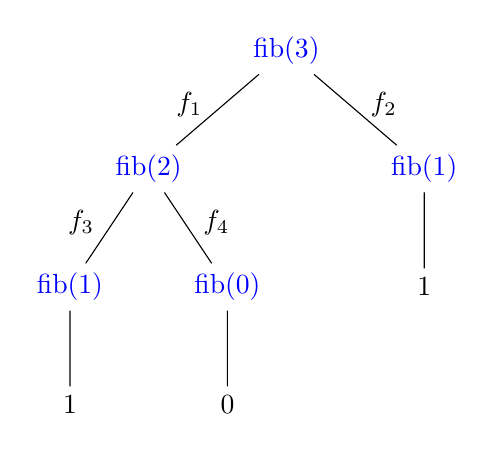
\begin{tikzpicture}[level distance=1.5cm,
level 1/.style={sibling distance=3.5cm},
level 2/.style={sibling distance=2cm}]
%\tikzstyle{every node}=[circle,draw]

\node (Root) [blue,rectangle] {fib(3)}
    child { node[blue] (q0) {fib(2)} 
      child { node[blue] (q00) {fib(1)}
        child { node[draw=none] {1} }
        edge from parent node [draw=none,left,xshift=-2.0,yshift=2.0] {$f_3$}
      }
      child { node[blue] (q01) {fib(0)} 
        child { node[draw=none] {0}         
        }
        edge from parent node [draw=none,right,xshift=2.0,yshift=2.0] {$f_4$}
      }
      edge from parent node [draw=none,left,xshift=-2.0,yshift=2.0] {$f_1$}
    }
    child { node [blue] (q1) {fib(1)}
      child { node[draw=none] (q10) {1}
      }
      edge from parent node [draw=none,right,xshift=2.0,yshift=2.0] {$f_2$}
    };
\end{tikzpicture}\caption{Breadth-first scheduling.}\label{fig:bfs}
\end{subfigure}
~
\begin{subfigure}[t]{0.5\textwidth}
\centering
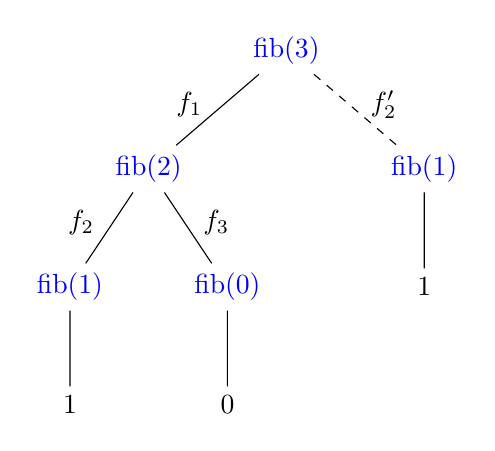
\begin{tikzpicture}[level distance=1.5cm,
level 1/.style={sibling distance=3.5cm},
level 2/.style={sibling distance=2cm}]
%\tikzstyle{every node}=[circle,draw]

\node (Root) [blue,rectangle] {fib(3)}
    child { node[blue] (q0) {fib(2)} 
      child { node[blue] (q00) {fib(1)}
        child { node[draw=none] {1} }
        edge from parent node [draw=none,left,xshift=-2.0,yshift=2.0] {$f_2$}
      }
      child { node[blue] (q01) {fib(0)} 
        child { node[draw=none] {0}         
        }
        edge from parent node [draw=none,right,xshift=2.0,yshift=2.0] {$f_3$}
      }
      edge from parent node [draw=none,left,xshift=-2.0,yshift=2.0] {$f_1$}
    }
    child[dashed] { node [blue] (q1) {fib(1)}
      child[solid] { node[draw=none] (q10) {1}
      }
      edge from parent node [draw=none,right,xshift=2.0,yshift=2.0] {$f_2'$}
    };
\end{tikzpicture}\caption{Depth-first scheduling. Note $f_2$ and $f_2'$ are disjoint tasks.}\label{fig:dfs}
\end{subfigure}\caption{Task labelled computation trees for \texttt{fib($3$)}.}
\end{figure*}

This scheduler is suboptimal for the Fibonacci-computation on single-core platform, because it unnecessarily materialises the entire computation tree of \texttt{fib($n$)}. Figure \ref{fig:bfs} depicts the computation tree for \texttt{fib($3$)}. The labels $f_i$ indicate tasks, and the subscripts $i$ their respective global id.

The scheduler fails to exploit the fact that a parent task depends on its two children tasks. We can remedy this issue by eagerly execute forked tasks. Visually, this policy to correspond to visiting the computation tree in a depth-first manner. Such a scheduler is similar to the \texttt{bfscheduler}, we only need to change queuing policy in the \texttt{Fork}-case, e.g.
\begin{lstlisting}[style={links},caption={}]
case Fork(t,k) -> {
 var new_f = new_future();
 enqueue(fun(_) { k(new_f)(f) });
 scheduler(t)(Just(new_f))()
}
\end{lstlisting}
Instead of enqueuing the forked task, we enqueue the continuation to run later. Moreover, we eagerly execute the forked task \texttt{t}.
Figure \ref{fig:dfs} depicts the labelled computation tree for \texttt{fib($3$)} when using this scheduler. Now, the entire computation tree no longer needs to materialised. The space used for tasks in the left subtree can be reused for subsequent tasks in the right subtree. Obviously, we save space, but it has a further subtle impact: The tasks yield fewer times which implies the scheduler is invoked fewer times. Thus, we reduced the overhead incurred by the scheduler. In the case of \texttt{fib($n$)} it means we, presumably, achieve a small improvement in performance.

Admittedly, the Fibonacci computation is trivial, and we are unlikely to encounter such a trivial computation in any practical application. However, the take away point from this example is, that, we were able change schedulers independently of the computation.

Essentially, we derived the sequential schedule for the naïve Fibonacci implementation. If we were to execute the computation on multicore platform, then the breadth-first scheduler would be a better choice. Fortunately, with this programming abstraction it is easy to change schedulers as computations and schedulers are expressed in the same language. In other words: We gain modularity.

\subsection{Proposal}
We propose to give an efficient implementation of effect handlers in the functional programming language Links.

\subsection{Project outcomes}
\begin{itemize}
  \item Efficient handlers.
  \item An account of concurrent programming with effect encoded concurrency.  
\end{itemize}

\section{Methodology}

  \section{Related work}\label{sec:relatedwork}
This section briefly summarises related work.

  \subsection{Concurrent and parallel programming models}
\begin{table*}
\centering
\begin{tabular}{| l | l | l |}
\hline
 \textbf{Language}             & \textbf{Programming model} & \textbf{Memory model}\\
\hline
CellSs, StarSs, StarPU, OpenMP & Annotations via pragmas; API & Shared memory \\
\hline
PaRSEC                         & Dataflow programming & Shared Memory \& Distributed memory  \\
\hline
MPI & Message-passing          & Distributed memory  \\
\hline
Unified Parallel C, Coarray Fortran & Shared variable programming & Partition Global Address Space \\
\hline
\end{tabular}
\caption{Classification of a selection of concurrent and parallel programming models.}\label{tbl:models}
\end{table*}
There exists numerous languages/tools that attempt to address the problem of scheduling in high-performance computing; a selection of these tools were briefly outlined in Section \ref{sec:problemdefinition}.

CellSs \cite{Bellens2009} provide a source-to-source compiler that translates annotated C or Fortran code. It attempts to automatically derive opportunities for task-based concurrency. StarSs \cite{Planas2009} and StarPU \cite{Augonnet2011} are influenced by CellSs. The former extends CellSs with hierarchical task scheduling. StarPU provides a unified platform for dynamic scheduling on heterogeneous multicore architectures. All three has influenced the open industry standard OpenMP \cite{Openmp2013}. 

PARSeC \cite{Bosilca2013} is a generic architecture-aware framework for task scheduling in heterogeneous environments. Programmers may implement their own schedulers using the PARSeC API. Schedulers operate on task dependency graphs which the runtime engine
Thus the runtime engine is aware of both the tasks to be executed and the dataflow which connects them.

\subsection{Multicore OCaml}
OCaml is a functional language with an industrial strength compiler. The Multicore OCaml project \cite{Dolan2015} attempts to bring multi-core capabilities to the OCaml language by using handlers to encode concurrency. The implementation of handlers is restricted to so-called \emph{linear handlers}, i.e. handlers which only invokes the continuation parameter once. However, this restriction is not enforced statically, therefore multiple invocations of a continuation result in a run-time error. Moreover, OCaml does not have an effect system.

\subsection{The Links intermediate representation}
The Links compiler uses A-normal form (ANF) as its intermediate representation for programs. ANF is the functional equivalent to the imperative Static Single Assignment form. All arguments to a function must be let-bound \cite{Flanagan1993}. This restriction makes it easy to build continuations.

  \subsection{Optimisation of single-shot continuations}

%   \subsection{Handlers implementations}
%   This section briefly surveys existing implementations of effect handlers. Section \ref{sec:first-class} considers languages with first-class handlers, whilst Section \ref{sec:library} discusses embeddings of handlers in the pure functional programming language Haskell.
%   \subsubsection{First-class implementations}\label{sec:first-class}
%   \begin{table}[H]
%     \centering 
%     \begin{tabular}{| l | l | l |}
%       \hline
%       \multicolumn{1}{|c|}{Language} & \multicolumn{1}{c|}{Handlers} & \multicolumn{1}{c|}{Developed by} \\
%       \hline
%       Eff & Deep handlers & Bauer and Pretnar \\ 
%       \hline
%       Frank & Shallow handlers & McLaughlin, Lindley and McBride \\    
%       \hline
%       Links & Shallow and deep handlers & Hillerström and Lindley\\
%       \hline
%       Multicore OCaml & Deep handlers & OCamlLabs \\
%       \hline    
%     \end{tabular}\caption{Languages with first-class effect handlers.}\label{tbl:impls}
%   \end{table}
%   Table \ref{tbl:impls} provide an overview of languages where effect handlers are first-class citizens. 

% The Eff language is a OCaml-style language with deep handlers. It support for effect polymorphism through subtyping \cite{Bauer2015}. 
% The functional programming Links implements both deep and shallow handlers \cite{Hillerstrom2015}. Moreover, the implementation supports effect polymorphism through Links' existing row polymorphic effect system.
    
%   \subsubsection{Library implementations}\label{sec:library}

  \section{Evaluation}
  The primary metric for evaluation of the proposed solution will be performance. As discussed earlier there are various metrics for measuring performance. We intend to mainly measure performance by raw execution speed. Furthermore, we intend to compare our performance results against results for similar programs written in C since it is considered a ``performant'' language. 

Additionally, we will consider the safety of our solution, i.e. which static guarantees, if any, can we exhibit. In order to evaluate safety we intend to give a formal proof of the said properties.

Furthermore, we would like to qualitatively assess the ease of use, that is, whether the handler abstraction makes concurrent programming easier.

  \section{Project plan}
  \begin{table}[H]
    \centering
    \begin{tabular}{ | l | c | c | c | c | c | }
      \hline
      \multicolumn{1}{|c|}{Activity / Weeks} & 2-4 & 5-9 & 10-17 & 18-21 & 22-33 \\
      \hline
      Prototyping    & X & X & & & \\
      \hline
      Implementation & X & X & X & X & X \\
      \hline
      Testing        & X & X & X & X & X \\
      \hline
      Evaluation     &   &   & X & X & X \\
      \hline
      Related work   &   & X & X &   & X \\
      \hline
      Exam period    &   &   &   & X &   \\
      \hline
      Write up       & X & X & X & X & X  \\
      \hline
    \end{tabular}\caption{Activity overview.}
  \end{table}
  % Bibliography
\bibliographystyle{abbrv}
\softraggedright
%\nocite{*}
\bibliography{references}
%  \printbibliography[heading=bibintoc]
\end{document}